% !TeX spellcheck = cs_CZ
%{\tikzset{external/prefix={tikz/FYZII/}}
% \tikzset{external/figure name/.add={ch20_}{}}
%---------------------------------------------------------------------------------------------------
% file fey2ch20.tex
%---------------------------------------------------------------------------------------------------
%=========================== Kapitola: Řešení Maxwellových rovnic ve volném prostoru  ==============
\setchaptertoc
\chapter{Řešení Maxwellových rovnic ve volném prostoru}\label{fyz:IIchapXX}

  \section{Vlny ve volném prostoru. Rovinné vlny}\label{fyz:IIchapXXsecI} 
  
    V kapitole \ref{fyz:IIchapXVIII} jsme se dostali k Maxwellovým rovnicím v úplném tvaru. Vše, co
    je možné se dozvédět o klasické teorii elektrických a magnetických polí, lze odvodit z těchto
    čtyř rovnic:
    \begin{equation}\label{fyz:eq963}
      \begin{alignedat}{3}
        &\text{I.}  &&\nabla\cdot \vec{E}          &\;=&\;\frac{\varrho}{\varepsilon_0}\\[1ex]
        &\text{II.} &&\nabla\times\vec{E}          &\;=&\;-\diffp{\vec{B}}{t}\\[1ex]
        &\text{III.}&&\nabla\cdot \vec{B}          &\;=&\;0\\[1ex]
        &\text{IV.}  &\quad c^2&\nabla\times\vec{B}&\;=&\;\frac{\vec{j}}{\varepsilon_0}+\diffp{\vec{E}}{t}
      \end{alignedat}
    \end{equation}

    Zkombinujeme-li všechny tyto rovnice, objeví se pozoruhodný jev: pole generovaná pohybujícími se
    náboji mohou opustit své zdroje a sama putovat prostorem. Uvažovali jsme speciální příklad, v
    němž náhle vznikl proud v nekonečném listu. Poté, co proud trval dobu \(t\) bylo vytvořeno
    homogenní elektrické pole, stejně jako homogenní magnetické pole a obě se šířila do vzdálenosti
    \(ct\) od zdroje. Předpokládejme, že list s proudem leží v rovině \(yz\) vztažné soustavy a má
    plošnou proudovou hustotu \(j\) ve směru kladné osy \(y\). Elektrické pole pak bude mít pouze
    \(y\)-ovou složku a magnetické pole pouze \(z\)-ovou složku. Velikosti obou složek vyjadřuje
    tento vztah:
    \begin{equation}\label{fyz:eq964}
      E_y=cB_z=-\frac{J}{2\varepsilon_0 c},
    \end{equation}
    pro kladné hodnoty \(x\) menší než \(ct\). Při větších \(x\) jsou pole rovna nule. Přirozeně,
    podobná pole se rozšířila do téže vzdálenosti od listu s proudem i ve směru záporné osy \(x\).
    Na obr. \ref{fyz:fig0643} vidíme graf velikosti polí jako funkce \(x\) v okamžiku \(t\). S
    postupem času se „čelo vlny“, které se v čase \(t\) nachází v polohách \(x = ct\), pohybuje
    konstantní rychlostí \(c\) k větším absolutním hodnotám \(x\).

    \begin{figure}[ht!] %\ref{fyz:fig0643}
      \centering
      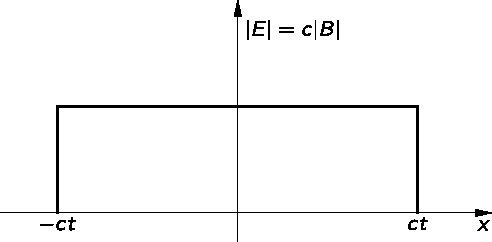
\includegraphics[width=0.7\linewidth]{fyz_fig0643.pdf}
      \caption{Elektrické a magnetické pole jako funkce \(x\) v čase \(t\) po tom, když začal téci
               proud. (\cite[s.~351]{Feynman02})}
      \label{fyz:fig0643}
    \end{figure}

    Nyní uvažujme následující posloupnost událostí. Zapněme na chvíli proud jednotkové velikosti,
    pak velikost proudu náhle zvětšme na tři jednotky a udržujme ji stále na této hodnotě.

    Jak budou vypadat pole v tomto případě? Můžeme to zjistit takto: Nejdříve si představíme jen
    proud o jednotkové velikosti, který byl spuštěn v čase \(t = 0\) a dále byl ponechán beze změny.
    Pole pro kladné \(x\) jsou v tomto případě graficky znázorněna v části a) obrázku
    \ref{fyz:fig0644}. Dále se ptáme, co se stane, zapneme-li v čase \(t_1\) ještě stálý proud o
    velikosti dvě jednotky.

    \begin{figure}[ht!]  %\ref{fyz:fig0644}
      \centering
      \subcaptionbox{proud velikosti jedné proudové jednotky byl spušněn v okamžiku \(t=0\) 
        \label{fyz:fig0644a}}{\luafigure[0.8]{fyz_fig0644a.pdf}} \\
      \subcaptionbox{proud velikosti dvou proudových jednotek byl spuštěn v okamžiku \(t=t_1\)
        \label{fyz:fig0644b}}{\luafigure[0.8]{fyz_fig0644b.pdf}} \\
      \subcaptionbox{superpozice případů a) a b) 
        \label{fyz:fig0644c}}{\luafigure[0.8]{fyz_fig0644c.pdf}}
      \caption{Elektrické pole listu s proudem (\cite[s.~351]{Feynman02})}
      \label{fyz:fig0644}
    \end{figure}

    V tomto případě budou pole dvakrát větší než předtím, ale rozšíří se ve směru osy \(x\) pouze do
    vzdálenosti \(c(t - t_1)\), což ukazuje část \ref{fyz:fig0644b} našeho obrázku. Když na základě
    principu superpozice tato dvě řešení sečteme, dostaneme výsledek, že součet obou zdrojů je roven
    proudu o jedné jednotce v čase od \(t=0\) do \(t=t_1\) a proudu o velikosti tři jednotky pro čas
    \(t\) větší než čas \(t_1\). V okamžiku \(t\) se budou pole ménit s \(x\) tak, jak to ukazuje
    část \ref{fyz:fig0644c}.

    \begin{figure}[ht!]  %\ref{fyz:fig0646}
      \centering
      \subcaptionbox{\label{fyz:fig0646a}}{\luafigure[0.8]{fyz_fig0646a.pdf}} \\
      \subcaptionbox{\label{fyz:fig0646b}}{\luafigure[0.8]{fyz_fig0646b.pdf}}
      \caption{Mění-li se intenzita proudu takovým způsobem, jaký udává graf a), průběh elektrického 
              pole v závislosti na \(x\) v okamžiku \(t\) vyznačeném šipkou znázorňuje graf b). 
              (\cite[s.~351]{Feynman02})}
      \label{fyz:fig0646}
    \end{figure}

    Nyní si vezměme složitější úlohu. Zkoumejme proud, který měl chvíli velikost jedné jednotky, pak
    vzrostl na tři jednotky a později klesl na nulu. Jaká pole vytvoří takovýto proud? Řešení můžeme
    najít týmž způsobem - sečtením řešení tří oddělených úloh. Nejdříve najdeme pole stupňovitého
    proudu s jednotkovou velikostí. (Tuto úlohu jsme již vyřešili.) Dále najdeme pole vytvářená
    stupňovitým proudem s velikostí dvě jednotky. Poté řešíme pole stupňovitého proudu s intenzitou
    minus tři jednotky. Když tato tři řešení sečteme, dostaneme proud, jehož velikost je od \(t =
    0\) do nějakého pozdějšího času, řekněme \(t_1\) rovna jedné jednotce, pak až do ještě
    pozdějšího okamžiku \(t_2\) třem jednotkám a nakonec je proud vypnut, to znamená, že dále je
    roven nule. Graf proudu jako funkci času ukazuje obr. \ref{fyz:fig0646a}. Sečteme-li všechna tři
    řešení pro elektrické pole, zjistíme, že jeho závislost od \(x\) v nějakém daném okamžiku (je
    znázorněna grafem na obr. \ref{fyz:fig0646b}. Pole je přesným obrazem proudu. Rozdělení pole v
    prostoru je vlastně krásným grafem závislosti proudu na čase - pouze narýsovaným odzadu. V čase
    se celý graf pohybuje rychlostí \(c\). Vznikla jakási malá hrudka pole, pohybující se ve směru
    kladné osy \(x\), která obsahuje úplně podrobnou informaci o historii všech proudových změn.
    Kdybychom stáli na míle daleko, mohli bychom ze změny elektrického nebo magnetického pole přesně
    rozpoznat, jak se proud ve zdroji měnil.

    Všimněme si také, že i když se celá činnost ve zdroji už dávno zastavila a všechny náboje a
    proudy jsou rovny nule, pokračuje blok pole nadále ve svém putování prostorem. Dostali jsme
    takové rozdělení elektrického a magnetického pole, které existuje nezávisle na jakýchkoliv
    nábojích nebo proudech. To je nový jev, který vyplývá z úplné soustavy Maxwellových rovnic.
    Je-li třeba, můžeme právě provedený rozbor kompletně vyjádřit i matematicky: napíšeme, že
    elektrické pole v daném místě a daném čase je přímo úměrné proudu ve zdroji, avšak ne v témže
    čase \(t\), ale v pozdějším čase \(t-\sfrac{x}{c}\). Můžeme tedy napsat
    \begin{equation}\label{fyz:eq965}
      E_y(t)=-\dfrac{J(t-\sfrac{x}{c})}{2\varepsilon_0 c}.
    \end{equation}
    Stejný vztah jsme už odvodili, věřte tomu nebo ne, z jiného hlediska v \ref{vol02:part:FYZI}.
    díle, když jsme se zabývali teorií indexu lomu. Tentokrát jsme zjišťovali, jaká pole vytváří
    tenká vrstva oscilujících dipólů nacházejících se v desce z dielekrtické látky, uvádí-li dipóly
    do pohybu elektrické pole dopadající elektromagnetické vlny. Naší úlohou bylo vypočítat, jak
    vypadají složená pole původní vlny a vln oscilujících dipólů. Jak jsme však mohli počítat pole
    generovaná pohybujícími se náboji, když jsme ještě neměli Maxwellovy rovnice? Tehdy jsme vzali
    jako východisko (bez jakéhokoliv odvozování) vzorec pro pole záření vytvářené ve velkých
    vzdálenostech od zrychleně se pohybujícího bodového náboje. Podíváme-li se do kapitoly
    \ref{vol02:fyz:IchapXXXI} v partii \ref{vol02:part:FYZI}, přesvědčíme se, že vztah
    \eqref{vol02:fyz:eq966} je přesně tentýž jako vztah \eqref{fyz:eq965}, který jsme právě napsali.
    Ačkoliv naše dřívější odvození platilo jen pro velké vzdálenosti od zdroje, nyní vidíme, že
    tentýž výsledek zůstává správný i v těsné blízkosti zdroje.

    Nyní se chceme obecně podívat na vlastnosti elektrických a magnetických polí ve vakuu, a to v
    oblastech vzdálených od zdrojů, tj. od proudů i nábojů. Velmi blízko u zdrojů (tak blízko, aby
    po dobu zpoždění v přenosu neměl zdroj dost času na větší změnu) se pole velmi podobají těm,
    kterájsme našli v elektromagnetických nebo magnetických případech. Vzdálíme-li se však
    dostatečně daleko, aby zpoždění byla významná, povaha polí se může od nalezených řešení
    radikálně lišit. V podstatě, když se pole vzdálila daleko od zdrojů, začínají získávat
    samostatný charakter. Proto jsme oprávněni začít hovořit o vlastnostech polí v oblasti, kde
    nejsou žádné proudy nebo náboje.
    
    Ptáme se, jaká pole mohou existovat v oblastech, kde jak \(\varrho\), tak i \(j\) jsou rovna
    nule. V kapitole \ref{fyz:IIchapXVIII} jsme viděli, že fyziku Maxwellových rovnic by bylo možné
    vyjádřit i pomocí diferenciálních rovnic pro skalární a vektorové potenciály:
    \begin{subequations}\label{fyz:eq967}
      \begin{align}      
        \nabla^2\varphi    - \dfrac{1}{c^2}\,\diffp[2]{\varphi}{t}
          &= -\dfrac{\varrho}{\varepsilon_0},      \label{fyz:eq967a} \\[1ex]     
        \nabla^2\vec{A} - \dfrac{1}{c^2}\,\diffp[2]{\vec{A}}{t}
          &= -\dfrac{\vec{j}}{\varepsilon_0c^2}.   \label{fyz:eq967b}
      \end{align}
    \end{subequations}
    Jsou-li \(\varrho\) a \(j\) rovna nule, získávají tyto rovnice jednodušší tvar:
    \begin{subequations}\label{fyz:eq968}
      \begin{align}      
        \nabla^2\varphi - \dfrac{1}{c^2}\,\diffp[2]{\varphi}{t}&= 0,   \label{fyz:eq968a} \\[1ex]     
        \nabla^2\vec{A} - \dfrac{1}{c^2}\,\diffp[2]{\vec{A}}{t}&= 0.   \label{fyz:eq968b}
      \end{align}
    \end{subequations}
    Ve vakuu tedy skalární potenciál \(\varphi\) jakož i každá složka vektorového potenciálu
    \(\vec{A}\), vyhovují téže matematické rovnici. Budeme psát \(\psi\) (psí) místo kterékoliv z
    těchto čtyř veličin: \(\varphi\), \(A_x\), \(A_y\), \(A_z\). Potřebujeme tedy prozkoumat obecná
    řešení následující rovnice:
    \begin{equation}\label{fyz:eq969}
      \nabla^2\psi - \dfrac{1}{c^2}\,\diffp[2]{\psi}{t}=0.
    \end{equation}
    Tato rovnice se nazývá \emph{trojrozměrná vlnová rovnice} (trojrozměrná proto, že funkce
    \(\psi\) může pbecně záviset na \(x\), \(y\) a \(z\) a musíme se zabývat změnou každé z těchto
    souřadnic). Toto se ihned ozřejmí, vypíšeme-li explicitně všechny tři členy Laplaceoya operátoru
    \(\nabla^2\):
    \begin{equation}\label{fyz:eq970}
      \diffp[2]{\psi}{x}+\diffp[2]{\psi}{y}+\diffp[2]{\psi}{z}-\frac{1}{c^2}\,\diffp[2]{\psi}{t}=0.
    \end{equation}

    Ve vakuu splňuji vlnovou rovnici i pole \(\vec{E}\) a \(\vec{B}\). Například protože \(\vec{B}=
    \nabla\times\vec{A}\), diferenciální rovnici pro \(\vec{B}\) můžeme dostat použitím operátoru
    rotace na rovnici \eqref{fyz:eq968b}. Laplaceův operátor je skalárním operátorem, proto je možné
    vzájemně zaměnit pořadí Laplaceova operátoru a operátoru rotace:
    \begin{equation*}
      \nabla\times\left(\nabla^2\vec{A}\right) 
        = \nabla^2\left(\nabla\times\vec{A}\right) 
        = \nabla^2\vec{B}.
    \end{equation*} 
    Podobně lze zaměnit i pořadí operátorů rotace a časové derivace \(\diffp{}{t}\)
    \begin{equation*}
      \nabla\times{\dfrac{1}{c^2}\,\diffp[2]{\vec{A}}{t}}
        = \dfrac{1}{c^2}\,\diffp[2]{}{t}\left(\nabla\times\vec{A}\right)
        = \dfrac{1}{c^2}\,\diffp[2]{\vec{B}}{t}.
    \end{equation*}
    Použitím těchto výsledků dostaneme následující diferenciální rovnici pro \(\vec{B}\):
    \begin{equation}\label{fyz:eq971}
      \nabla^2\vec{B} - \frac{1}{c^2}\,\diffp[2]{\vec{B}}{t}=0.
    \end{equation}
    Každá složka magnetického pole \(\vec{B}\) tedy splňuje trojrozměrnou vlnovou rovnici. Podobně
    použitím vztahu \(\vec{E}=-\nabla{\varphi}-\diffp{\vec{A}}{t}\) vyplyne, že i elektrické pole
    \(\vec{E}\) ve vakuu splňuje rovnici:
    \begin{equation}\label{fyz:eq972}
      \nabla^2\vec{E} - \frac{1}{c^2}\,\diffp[2]{\vec{E}}{t}=0.
    \end{equation}
    Všechna naše elektromagnetická pole vyhovují tedy téže jedné rovnici \eqref{fyz:eq970}. Bylo by
    možné se zeptat: Co je nejobecnějším řešením této rovnice? Avšak místo toho, abychom se hned
    vydali hledat odpověď na tuto obtížnou otázku, se nejdříve podíváme, co lze obecně říci o těch
    řešeních, v nichž se podle \(y\) a \(z\) nic nemění. (Vždy se pusťme nejdříve do lehkého
    příkladu, abychom měli možnost pochopit, o co vůbec jde, a pak můžeme přejít k případům
    složitějším.) Předpokládejme tedy, že velikosti polí závisí jen na \(x\), \(y\), tj. že s \(y\)
    a \(z\) se pole nemění. Uvažujeme tedy opět rovinné vlny. Můžeme očekávat, že dostaneme nějaké
    podobné výsledky jako dříve. Opravdu, najdeme přesně tytéž výsledky. Můžeme se ptát: „Proč se to
    tedy dělá všechno znovu?“ Udělat to znovu je důležité, za prvé proto, že jsme neukázali, že námi
    nalezené vlny představují nejobecnější řešení pro rovinné vlny a za druhé proto, že pole jsme
    našli pouze na základě velmi zvláštního druhu zdroje s proudem. Nyní bychom si rádi položili
    otázku: Jak vypadá nejobecnější druh jednorozměrného vlnění, které může existovat ve vakuu?
    “Nelze to zjistit tak, že budeme zkoumat, co se děje v případě toho nebo onoho konkrétního
    zdroje, ale musíme pracovat obecněji. Kromě toho budeme tentokrát pracovat s diferenciálními
    rovnicemi místo integrálních tvarů. I když dostaneme stejné výsledky, jde o to, abychom se
    trochu procvičili a přesvědčili se, že nezáleží na tom, kterou cestou vlastně jdeme. Měli bychom
    umět postupovat jakýmkoliv způsobem, neboť dostanete-li těžký problém, často zjistíme, že ho
    lze zvládnout pouze jedním z rozmanitých způsobů.
    
    Mohli bychom zkoumat přímo řešení vlnové rovnice pro některou elektromagnetickou veličinu. Místo
    toho však chceme vyjít ze samotného začátku, tj. z Maxwellových rovnic pro vakuum, abychom měli
    možnost vidět jejich těsnou souvislost s elektromagnetickými vlnami. Začneme tedy s rovnicemi
    \eqref{fyz:eq963}, v nichž položíme náboje a proudy rovny nule. Rovnice pak získají tento tvar:
    \begin{equation}\label{fyz:eq973}
      \begin{alignedat}{3}
        &\text{I.}  &&\nabla\cdot \vec{E}          &\;=&\;0\\[1ex]
        &\text{II.} &&\nabla\times\vec{E}          &\;=&\;-\diffp{\vec{B}}{t}\\[1ex]
        &\text{III.}&&\nabla\cdot \vec{B}          &\;=&\;0\\[1ex]
        &\text{IV.}  &\quad c^2&\nabla\times\vec{B}&\;=&\;\diffp{\vec{E}}{t}
      \end{alignedat}
    \end{equation}
    Vypíšeme první rovnici ve složkách:
    \begin{equation}\label{fyz:eq974}
      \nabla\cdot\vec{E}=\diffp{E_x}{x}+\diffp{E_y}{y}+\diffp{E_z}{z}=0.
    \end{equation}
    Předpokládáme, že podle \(y\) a \(z\) žádné změny nenastávají, takže poslední dva členy jsou
    rovny nule. Proto podle této rovnice
    \begin{equation}\label{fyz:eq975}
      \diffp{E_x}{x}=0.
    \end{equation}
    Jejím řešením je v prostoru konstantní \(E_x\) - složka elektrického pole ve sméru osy \(x\).
    VŠimneme-li si rovnice IV v \eqref{fyz:eq973}, přičemž předpokládáme, že podle \(y\) a podle
    \(z\) k žádným zménám \(\vec{B}\) nedochází, vidíme, že \(E_x\) je konstantní i v čase. Takovým
    polem by mohlo být ustálené pole vytvářené elektrodami nějakého velmi vzdáleného nabitého
    kondenzátoru. Nyní se však o takové nezajímavé statické pole nestaráme; zajímají nás jen
    dynamicky proměnná pole. A v \emph{dynamických} polích je \(E_x=0\).
    
    Dostali jsme tak důležitý výsledek, že při šíření rovinných vln v libovolném směru \emph{musí
    být elektrické pole kolmé na směr šíření}. Přitom se ovšem může ještě všelijak složitě měnit se
    souřadnicí \(x\).
    
    Příčné pole \(\vec{E}\) lze vždy rozložit na dvě složky, řekněme na \(y\)-ovou a na \(z\)-ovou.
    Proto probereme především případ, kdy má elektrické pole jen jednu příčnou složku. Budeme
    zkoumat nejdříve elektrické pole, které má vždy směr osy \(y\), a tedy nulovou \(z\)-ovou
    složku. Zřejmě, rozšíříme-li tuto úlohu, můžeme vždy vyřešit i případ, kdy elektrické pole leží
    vždy ve směru osy \(z\). Obecné řešení lze pak vyjádřit jako superpozice těchto dvou polí.
    
    Jak jednoduché jsou nyní naše rovnice! Jedinou nenulovou složkou elektrického pole je \(E_y\) a
    všechny derivace - s výjimkou těch, které jsou podle \(x\) - jsou rovny nule. Ostatní Maxwellovy
    rovnice se tím podstatně zjednodušují.
    
    Všimněme si dále druhé z Maxwellových rovnic (II v \eqref{fyz:eq973}). Vypíšeme-li složky
    \(\rot{E}\), dostaneme
    \begin{alignat*}{4}
      &\left(\nabla\times\vec{E}\right)_x&&=\diffp{E_z}{y}&&-\diffp{E_y}{z}&&=0,\\[1.5ex]
      &\left(\nabla\times\vec{E}\right)_y&&=\diffp{E_x}{z}&&-\diffp{E_z}{x}&&=0,\\[1.5ex]
      &\left(\nabla\times\vec{E}\right)_z&&=\diffp{E_y}{x}&&-\diffp{E_x}{y}&&=\diffp{E_y}{x}.
    \end{alignat*}
    \(x\)-ová složka vektoru \(\left(\nabla\times\vec{E}\right)\) je rovna nule, neboť jsou rovny
    nule derivace podle \(y\) i podle \(z\). Složka \(y\)-ová je také rovna nule: první člen je
    roven nule, neboť derivace podle \(z\) je rovna nule, a druhý člen je roven nule, neboť \(E_z\)
    je rovno nule. Jedinou nenulovou složkou vektoru \(\rot{E}\) je \(z\)-ová složka, která je rovna
    \(\diffp{E_y}{x}\). Položíme-li tyto tři složky \(\nabla\times\vec{E}\) položíme rovny
    příslušným složkám vektoru \(-\diffp{\vec{B}}{t}\), můžeme udélat následující závéry:
    \begin{subequations}\label{fyz:eq977} 
      \begin{align}
        &\diffp{B_x}{t}=0,\quad\diffp{B_y}{t}=0. \label{fyz:eq977a} \\[1ex]
        &\diffp{B_z}{t}=-      \diffp{E_y}{x}.   \label{fyz:eq977b} 
      \end{align}     
    \end{subequations}

    Protože \(x\)-ová, jakož i \(y\)-ová složka magnetického pole, mají nulové derivace podle času,
    představují obě tyto složky pouze konstantní pole a odpovídají magnetostatickým řešením, které
    jsme našli předtím. Někdo mohl zanechat nějaké permanentní magnety v blízkosti místa, jímž se
    šíří vlny. My tato konstantní pole budeme ignorovat a položíme \(B_x\) a \(B_y\) rovny nule.
    
    Mimochodem k tomu, že \(x\)-ová složka pole \(\vec{B}\) musí být rovna nule jsme došli i jiným
    způsobem. Protože divergence \(\vec{B}\) je nulová (podle třetí Maxwellovy rovnice), stejnými
    úvahami, které jsme udělali pro elektrické pole, bychom usoudili, že podélná složka magnetického
    pole se nemůže měnit se souřadnicí \(x\). Protože takové homogenní pole v našich vlnových
    řešeních ignorujeme, museli bychom položit rovno nule \(\vec{B}\). V případě rovinných
    elektromagnetických vln tedy musí pole \(B_y\) jakož i pole \(\vec{E}\) být kolmé na směr šíření
    vln.
    
    Rovnice \eqref{fyz:eq977b} nám poskytuje dodatečný argument pro závěr, že má-li elektrické pole
    jen složku \(y\), bude mít magnetické pole jen složku \(z\). Pole \(\vec{E}\) a \(\vec{B}\) jsou
    tedy navzájem kolmá. To je přesně to, co nastává v případě speciální vlny, kterou jsme již
    zkoumali.
    
    Nyní jsme připraveni k použití poslední z Maxwellových rovnic pro vakuum [IV v
    \eqref{fyz:eq973}]. Jejím rozepsáním do složek dostaneme:
    \begin{equation}\label{fyz:eq978}
      \begin{alignedat}{4}
        &c^2\left(\nabla\times\vec{B}\right)_x&&=
          c^2\,\diffp{B_z}{y}&&-c^2\,\diffp{B_y}{z}&&=\diffp{E_x}{t},\\[1ex]
        &c^2\left(\nabla\times\vec{B}\right)_y&&=
          c^2\,\diffp{B_x}{z}&&-c^2\,\diffp{B_z}{x}&&=\diffp{E_y}{t},\\[1ex]
        &c^2\left(\nabla\times\vec{B}\right)_z&&=
          c^2\,\diffp{B_y}{x}&&-c^2\,\diffp{B_x}{y}&&=\diffp{E_z}{t}.
      \end{alignedat}
    \end{equation}
    Ze šesti derivací složek vektoru \(\vec{B}\) není rovna nule pouze \(\diffp{B_z}{x}\). Proto z
    těchto tří rovnic nakonec dostaneme pouze vztah:
    \begin{equation}\label{fyz:eq979}
      -c^2\,\diffp{B_z}{x}=\diffp{E_y}{t}.
    \end{equation}

    Výsledek celé naší práce spočívá v závěru, že jen jedna složka elektrického a jen jedna složka
    magnetického pole není rovna nule a že tyto složky musí splňovat rovnice \eqref{fyz:eq977b} a
    \eqref{fyz:eq979}. Obě tyto rovnice lze zkombinovat do jediné, zderivujeme-li první podle \(x\)
    a druhou podle \(t\). Pak budou levé strany obou rovnic identické (až na součinitel \(c^2\)).
    Dostaneme tak, že \(E_y\) vyhovuje rovnici
    \begin{equation}\label{fyz:eq980}
      \diffp[2]{E_y}{x}-\dfrac{1}{c^2}\,\diffp[2]{E_y}{t}=0.
    \end{equation}
    která už se nám vyskytla dříve, když jsme zkoumali šíření zvuku. Je to vlnová rovnice pro
    jednorozměrné vlny.

    Všimněme si, že v procesu našeho odvozování jsme našli ještě něco víc, než obsahuje rovnice
    \eqref{fyz:eq972}. Maxwellovy rovnice nám poskytly další informaci, která spočívá v tom, že v
    elektromagnetických vlnách mají pole nenulové složky jen ve směrech kolmých na směr postupu
    vlnění.
    
    Shrňme si, co víme o řešeních jednorozměrné vlnové rovnice. Splňuje-li nějaká veličina
    \(\psi\) jednorozměrnou vlnovou rovnici
    \begin{equation}\label{fyz:eq981}
      \diffp[2]{\psi}{x}-\dfrac{1}{c^2}\,\diffp[2]{\psi}{t}=0,
    \end{equation}
    je jediným možným řešením funkce \(\psi(x, t)\), která má tvar
    \begin{equation}\label{fyz:eq982}
      \psi(x,t)=f(x-ct),
    \end{equation}
    tj. funkce jediné proměnné \((x - ct)\). Funkce \(f(x- ct)\) představuje nějaký „tuhý“ (v
    závislosti na \(x\)) útvar, který se pohybuje rychlostí \(c\) ve směru zvětšování kladných
    hodnot \(x\) (obr. \ref{fyz:fig0647}), Například, má-li funkce \(f\) maximum tehdy, když je její
    argument roven nule, pro \(t=0\) bude mít \(\psi\) maximum v \(x = 0\). V nějakém pozdějším
    čase, dejme tomu \(t= 10\), bude mít \(\psi\) maximum v \(x=10c\). S postupem času se maximum
    pohybuje rychlostí \(c\) ve směru kladné osy \(x\).

    \begin{figure}[ht!] %\ref{fyz:fig0647}
      \centering
      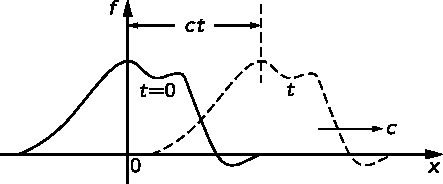
\includegraphics[width=0.9\linewidth]{fyz_fig0647.pdf}
      \caption{Funkce \(f(x-ct)\) představuje stálý „profil“, který se pohybuje rychlostí \(c\) ve
               směru nárůstu kladných hodnot \(x\). (\cite[s.~357]{Feynman02})}
      \label{fyz:fig0647}
    \end{figure}

    Někdy je vhodnější říkat, že řešení jednorozměrné vlnové rovnice je funkcí \((t -
    \sfrac{x}{c})\). Toto vyjádření však znamená totéž, co předcházející, neboť každá funkce v
    argumentu \((t - \sfrac{x}{c})\) je zároveň funkcí argumentu \((x - ct)\):
    \begin{equation*}
      F\left(t-\sfrac{x}{c}\right)=F\left[-\dfrac{x-ct}{c}\right]=f(x-ct).
    \end{equation*}

    Dokážeme, že \(f(x - ct)\) je opravdu řešením vlnové rovnice. Protože jde o funkci pouze jediné
    proměnné - proměnné \((x - ct)\) - budeme první derivaci \(f\) podle této proměnné označovat
    \(f'\) a druhou \(f''\). Derivováním vztahu \eqref{fyz:eq982} podle \(x\) dostaneme
    \begin{equation*}
      \diffp{\psi}{x}=f'(x-ct),
    \end{equation*}
    neboť derivace \((x - ct)\) podle \(x\) je rovna 1. Je zřejmé, že druhá derivace podle \(x\)
    bude
    \begin{equation}\label{fyz:eq983}
      \diffp[2]{\psi}{x}=f''(x-ct).
    \end{equation}
    Derivováním \(\psi\) podle \(t\) dostaneme
    \begin{align}
      &\diffp{\psi}{t}=f'(x-ct)(-c),  \notag\\[1.5ex]
      &\diffp{\psi}{t}=+c^2f''(x-ct). \label{fyz:eq984}
    \end{align}
    Vidíme, že \(\psi\) opravdu splňuje jednorozměrnou vlnovou rovnici.

    Můžete namítnout: „Mám-li vlnovou rovnici, odkud vím, že mám vzít právě \(f(x- ct)\) jako její
    řešení? Mně se tato zpětná metoda důkazu nelíbí. Neexistuje nějaký přímý způsob, jak dojít k
    řešení?“ V pořádku, jediným dobrým přímým způsobem je znát řešení. Je možné vymyslet nějaký
    zjevně přímý matematický postup, zvláště proto, že víme, jak má vlastně řešení vypadat, ale s
    rovnicí tak jednoduchou jako je tato, si nemusíme hrát na schovávanou. Téměř se dostaneme do
    stavu, že když uvidíme rovnici \eqref{fyz:eq981}, téměř současně se nám vybaví \(\psi=f(x- ct)\)
    jako její řešení. (Právě tak jako teď, když vidíme integrál \(x^2\dd{x}\), ihned víme, že
    výsledek je \(\sfrac{x^3}{3}\)).
    
    Ve skutečnosti byste měli vědět ještě trochu víc. Řešením je nejen každá funkce proměnné \((x -
    ct)\), ale i každá funkce proměnné \((x + ct)\). Protože vlnová rovnice obsahuje pouze \(c^2\),
    nehraje změna znaménka u \(c\) žádnou roli. Opravdu nejobecnějším řešením jednorozměrné vlnové
    rovnice je součet dvou libovolných funkcí, z toho jedné funkce proměnné \((x - ct)\) a druhé
    funkce proměnné \((x + ct)\):
    \begin{equation}\label{fyz:eq985}
      \psi=f(x - ct)+g(x + ct).
    \end{equation}

    První člen představuje nějakou vlnu postupující ve směru kladné osy \(x\) a druhý člen
    libovolnou vlnu postupující ve směru záporných hodnot \(x\). Obecné řešení je superpozicí obou
    takových současně existujících vln.
    
    Následující zábavný problém zatím řešit nebudeme, ale jen naznačíme jeho řešení. Vezměme funkci
    tvaru
    \begin{equation*}
      \psi=\cos kx\cos kct.
    \end{equation*}
    Tato funkce nemá tvar funkce proměnné \((x - ct)\) nebo \((x + ct)\). Naproti tomu můžeme jejím
    přímým dosazením do rovnice \eqref{fyz:eq981} snadno dokázat, že je řešením vlnové rovnice. Jak
    potom můžeme tvrdit, že obecné řešení má tvar vyjádřený vztahem \eqref{fyz:eq985}?
    
    Aplikujeme-li naše závěry o řešení vlnové rovnice na \(y\)-ovou složku elektrického pole
    \(E_y\), dojdeme k závěru, že \(E_y\) se může měnit s \(x\) jakýmkoliv způsobem. Avšak pole,
    která opravdu existují, lze vždy považovat za součet dvou útvarů. Jedna vlna putuje prostorem
    rychlostí \(c\) v jednom směru, přičemž s ní související magnetické pole je kolmé na elektrické
    pole; druhá vlna postupuje toutéž rychlostí opačným směrem. Takové vlny odpovídají nám už známým
    elektromagnetickým vlněním - světlu, radiovým vlnám, infračervenému záření, ultrafialovému
    záření, rentgenovým paprskům atd. O vyzařování světla jsme už podrobně hovořili v partii
    \ref{vol02:part:FYZI}. Protože všechno, co jsme se tam dozvěděli, platí pro každé elektromagnetické
    vlnění, není třeba zde podrobněji zkoumat vlastnosti těchto vln.
    
    Snad bychom měli udělat ještě několik poznámek o problému polarizace elektromagnetických vln. V
    našem řešení jsme se rozhodli zkoumat speciální případ, v němž má elektrické pole pouze složku
    \(y\). Pro vlny postupující ve směru \(+x\) nebo \(-x\) zřejmě existuje i jiné řešení, a to
    takové, které má pouze složku \(z\). Protože Maxwellovy rovnice jsou lineární, představuje
    obecné řešení v případě jednorozměrného vlnění postupujícího ve směru osy \(x\) součet vln
    \(E_y\) a vln \(E_z\). Toto obecné řešení shrnují následující vztahy:
    \begin{equation}\label{fyz:eq986}
      \begin{aligned}
        \vec{E}   &=(0,E_y,E_z)            \\[.5ex]
        E_y       &=f(x-ct)+g(x+ct)        \\[.5ex]
        E_z       &=F(x-ct)+G(x+ct)        \\[1ex]
        \vec{B}   &=(0,B_y,B_z)            \\[.5ex]
        cB_z      &=f(x-ct)-g(x+ct)        \\[.5ex]
        cB_y      &=-F(x-ct)+G(x+ct).
      \end{aligned}
    \end{equation}
    V takových elektromagnetických vlnách není směr vektoru \(\vec{E}\) konstantní, ale nějakým
    libovolným způsobem krouží v rovině \(yz\). Magnetické pole v každém bodě je vždy kolmé na
    elektrické pole a na směr šíření vlnění.
    
    Máme-li pouze vlny postupující jedním směrem, řekněme ve směru kladné osy \(x\), existuje pro
    orientaci elektrického a magnetického pole jednoduché pravidlo. Podle něj vektorový součin
    \(\vec{E} \times \vec{B}\) - což je ovšem vektor kolmý jak na \(\vec{E}\) tak i na \(\vec{B}\) -
    udává směr postupu vlnění. Ztotožní-li se tedy \(\vec{E}\) s \(\vec{B}\) pootočením doprava, tj.
    tak jako se zavrtává šroub s pravotočivým závitem, je směr posunu šroubu směrem rychlosti
    vlnění. (Později uvidíme, že vektor \(\vec{E} \times \vec{B}\) má speciální fyzikální význam. Je
    to vektor, který popisuje tok energie v elektromagnetickém poli.)

  \section{Trojrozměrné vlny}\label{fyz:IIchapXXsecII}    
    Nyní se pustíme do problému trojrozměrných vln. Už jsme viděli, že vektor \(\vec{E}\) vyhovuje
    vlnové rovnici. K témuž závěru lze snadno dojít i úvahou vycházející přímo z Maxwellových
    rovnic. Vyjděme z rovnice
    \begin{equation*}
      \nabla\times\vec{E}=-\diffp{\vec{B}}{t}
    \end{equation*}
    a na obě její strany aplikujme operátor rotace:
    \begin{equation}\label{fyz:eq987}
      \nabla\times(\nabla\times\vec{E}) = -\diffp{}{t}(\nabla\times\vec{B}).
    \end{equation}
    Jistě si vzpomínáme, že rotace každého vektoru lze psát jako součet dvou členů - jednoho
    obsahujícího divergenci a druhého obsahujícího Laplaceův operátor:
    \begin{equation*}
      \nabla\times(\nabla\times\vec{E})= \nabla(\nabla\cdot\vec{E})-\nabla^2\vec{E}.
    \end{equation*}
    Ve vakuu je však divergence \(\vec{E}\) rovna nule, takže zůstává laplaceovský člen. Kromě toho
    podle čtvrté z Maxwellových rovnic \eqref{fyz:eq973} je časová derivace \(c^2(\nabla \times
    \vec{B})\) rovna druhé derivaci \(\vec{E}\) podle času \(t\):
    \begin{equation*}
      c^2\,\diffp{}{t}(\nabla\times\vec{B})=\diffp[2]{\vec{E}}{t}.
    \end{equation*}
    Potom rovnice \eqref{fyz:eq987} získává tvar
    \begin{equation*}
      \nabla^2\vec{E} = \dfrac{1}{c^2}\,\diffp[2]{\vec{E}}{t},
    \end{equation*}
    který představuje trojrozměrnou vlnovou rovnici. Napsaná v celé své nádheře má tuto formu
    \begin{equation}\label{fyz:eq988}
      \diffp[2]{\vec{E}}{x}+\diffp[2]{\vec{E}}{y}+\diffp[2]{\vec{E}}{z}-
      \frac{1}{c^2}\,\diffp[2]{\vec{E}}{t}=0.
    \end{equation}

    Jak najdeme obecné řešení této vlnové rovnice? Všechna řešení trojrozměrné vlnové rovnice lze
    vyjádřit jako superpozice námi už nalezených jednorozměrných řešení. Když jsme předpokládali, že
    pole nezávisí na \(y\) a na \(z\), dostali jsme rovnici pro vlny postupující ve směru osy \(x\).
    Zřejmě existují i jiná řešení, v nichž pole nezávisí na \(x\) a \(y\) a reprezentují vlny
    pohybující se ve směru osy \(z\). Nebo obecně, protože jsme naše rovnice psali ve vektorovém
    tvaru, může mít trojrozměrná vlnová rovnice řešení, která znamenají rovinné vlny postupující v
    jakémkoliv směru. A opět, protože jde o lineární rovnice, můžeme mít současně rovinných vln,
    kolik jen chceme a šířit se mohou právě tolika směry. Nejobecnějším řešením trojrozměrné vlnové
    rovnice je tedy superpozice všech druhů rovinných vln pohybujících se všemi možnými směry.
    
    Zkuste si představit, jak vypadají elektrická a magnetická pole právě teď v prostoru této
    posluchárny. Především je tu stálé magnetické pole pocházející z elektrických proudů uvnitř
    Země, tj. stálé zemské magnetické pole. Jsou tu i určitá nepravidelná, ale téměř statická
    elektrická pole, která vznikají třeba od elektrických nábojů generovaných třením, když se lidé
    vrtí na svých židlích, nebo třou rukávy svých kabátů o jejich opěradla. Existují tu i další
    magnetická pole vytvářená střídavými proudy v elektrickém vedení. Tato pole se mění s frekvencí
    \qty{60}{\Hz}, synchronně s otáčením generátorů v elektrárně. Nejzajímavější jsou však ta
    elektrická a magnetická pole, která se mění s mnohem většími frekvencemi. Například když světlo
    prochází od okna na podlahu, od stěny ke stěně, vzniká drobné chvění elektrických a magnetických
    polí, které se šíří rychlostí \num{300000} kilometrů za sekundu. Dále existují ještě
    infračervené vlny dopadající na chladnou tabuli od našich rozpálených čel. A to jsme ještě
    zapomněli na ultrafialové záření, rentgenové paprsky a radiové vlny pronikající místností.
    
    Naší posluchárnou proletují elektromagnetické vlny přenášející hudbu džezové kapely. Existují
    zde vlny modulované sériemi impulzů, představující obrazy událostí, k nimž dochází v jiných
    částech světa nebo v nás samotných. Pro demonstraci reálnosti těchto vlnění je třeba pouze
    zapnout elektronické zařízení, které tyto vlny změní na obrazy a zvuky.

    \luagraphic[1]{fyz_fig0654.jpg}{Mariner 2 byla první úspěšná meziplanetární kosmická loď na
      světě. Spuštěn 27. srpna 1962 na raketě Atlas-Agena, Mariner 2 prošel asi 34 000 kilometrů od
      Venuše a poslal zpět cenné nové informace o meziplanetárním prostoru a atmosféře Venuše.
      Mariner 2 poprvé zaznamenal teplotu na Venuši a odhalil velmi horkou atmosféru planety asi
      \qty{500}{\degreeCelsius}. Sonda také poprvé měřila hustotu, rychlost, složení a kolísání
      solárního větru v čase. Kredit: Wikipedia}{fyz:fig0654}
    
    Půjdeme-li ještě do dalších podrobností a budeme analyzovat i nejmenší chvění, existují v této
    místnosti ještě velmi slabé elektromagnetické vlny, jež sem přišly z obrovských vzdáleností.
    Jsou zde také drobné oscilace elektrického pole, jejichž amplitudy jsou vzdálené zhruba
    \qty{30}{\cm}. Přišly z míst vzdálených od nás miliony kilometrů a byly k Zemi vyslány kosmickou
    sondou \textsc{Mariner 2}, která právě proletěla kolem Venuše\footnote{Dne 14. prosince 1962
    proletěla kolem planety Venuše (\qty{34752}{\km} od povrchu)}. Její signály nesou souhrn
    informací získaných sondou o této planetě (informaci jí dodaly elektromagnetické vlny, které
    sonda přijala od planety).
    
    Existují zde i velmi slabé kmity elektrických a magnetických polí - vlny, které pocházejí z míst
    vzdálených od nás miliardy světelných let, od galaxií v nejvzdálenějších koutech vesmíru. Že je
    tomu opravdu tak, bylo zjištěno „zaplněním místnosti vodiči“, tj. vybudováním velkých antén,
    jako je tato místnost. Jimi se detekovaly radiové vlny, které pocházejí z míst, ležících ve
    vesmíru za hranicí viditelnosti i těch největších optických teleskopů. Ostatně i ty, optické
    teleskopy, jsou v podstatě jen sběrači elektromagnetických vln. To co nazýváme hvězdami, jsou
    jen závěry - závěry udělané na základě pouze jediné fyzikální reality, kterou jsme z nich až
    dosud dostali - na základě výzkumu nekonečně složitých vlnění elektrických a magnetických polí,
    které zasahují naši Zem.
    
    Je toho ještě víc: pole vytvářená na míle vzdálenými blesky, pole nabitých částic v kosmickém
    záření, když sviští touto místností, a další a další. Vidíme, jakým složitým objektem je
    elektrické pole v prostoru kolem nás. Ale i tak vždy splňuje trojrozměrnou vlnovou rovnici.

  \section{O Vědecké obrazotvornosti}\label{fyz:IIchapXXsecIII} 
  
    Cco bychom měli při pokusu představování si elektrických a magnetických polí vlastně dělat? Víme
    vůbec jak na to? Jak si představovat elektrické a magnetické pole? Jaké jsou vůbec požadavky na
    \emph{vědeckou představivost}? Liší se něčím od pokusu představit si, že tato místnost je plná
    neviditelných andělů? Ne, nepodobá se představování si neviditelných andělů. Pochopit
    elektromagnetické pole vyžaduje mnohem vyšší stupeň představivosti než pochopit neviditelné
    anděly. Proč? Protože vše, co musíme udělat proto, abychom učinili neviditelné anděly dostupné
    chápání, je pouze trochu změnit jejich vlastnosti - udělám je trochu viditelné a už mám možnost
    vidět obrysy jejich křídel, jejich těla, svatozáře. Jakmile se mi už podařilo představit si
    viditelného anděla, je abstrakce potřebná k tomu, abychom si z téměř neviditelných andělů
    vytvořili představu o docela neviditelných, poměrně snadná. Asi řekneme, že stačí požádat pana
    profesora na přednášce: „Profesore, dejte nám, prosím, přibližný popis elektromagnetických vln,
    třeba ne úplně přesný, abychom je mohli vidět stejně tak, jako můžeme vidět téměř neviditelné
    anděly. Pak si budeme moci upravit obraz potřebnou abstrakcí.“
    
    Bohužel, tak to nefunguje. Není žádný obraz tohoto elektromagnetického pole, který by byl v
    nějakém ohledu přesný. Feynman napsal: \uv{O elektromagnetickém poli vím už dávno - byl jsem ve
    stejné situaci, jako jste nyní vy, před dvaceti pěti lety a mám už za sebou 25 roků přemýšlení o
    těchto třepotajících se vlnách. Když jsem začal s popisem magnetického pole pohybujícího se
    prostorem, mluvil jsem o polích \(\vec{E}\) a \(\vec{B}\) a mával jsem při tom rukama a vy se
    snad domníváte, že jsem opravdu schopný je vidět. Povím vám co vidím. Vidím jakési nejasné,
    zastíněné, třepotající se čáry - tu a tam je na nich nějak napsané \(\vec{E}\) a \(\vec{B}\),
    tu a tam jsou některé z těchto čar označeny šipkami - šipka mizí, když se na ni pozorněji
    podívám. Hovořím-li o polích, která se ženou prostorem, úžasně se pletou symboly, které používám
    k popisu objektů, s objekty samotnými. Ve skutečnosti si nedokážu vytvořit nějaký obraz, který
    se alespoň přibližně podobá reálným vlnám. Máte-li tedy i vy určité těžkosti s vytvořením
    takového obrazu, nemusíte se obávat, že vaše těžkosti jsou něco výjimečného}.
    
    Věda klade úžasné požadavky na představivost. Stupeň představivosti, jenž je vyžadován dnes, je
    mnohem větší než ten, který si nárokovali ze starodávných představ. Moderní pojmy se velmi těžko
    představují. Je pravda, že k tomu používáme mnohé prostředky. Používáme matematické rovnice a
    pravidla a děláme mnoho obrázků. Teď si uvědomuji, že když hovořím o elektromagnetickém poli v
    prostoru, vidím nějakou superpozici všech grafů, které jsem kdy viděl o těchto polích
    nakreslené. Před mým zrakem nejsou svazky siločar táhnoucí se prostorem, neboť mě trápí, že
    kdybych se pohyboval jinou rychlostí, tyto svazky by zmizely. Ani vždy nevidím elektrická a
    magnetická pole, neboť se někdy domnívám, že bych si měl svou představu vytvořit raději pomocí
    vektorového a skalárního potenciálu, neboť ty snad byly fyzikálně významnějšími realitami, které
    oscilovaly.
    
    Můžeme se domnívat, že asi jedinou nadějí je přijmout matematické hledisko. Jaké je tedy
    matematické hledisko? Z matematického hlediska existuje v každém bodě prostoru vektor
    elektrického pole, jakož i vektor magnetického pole; to však znamená, že s každým bodem je
    spojeno šest čísel. Dokážete si představit šest čísel spojených s každým bodem v prostoru? Velmi
    těžko. Dokážete si představit byť jen jedno číslo spojené s každým bodem? Já ne. Umím si
    představit takovou věc jakou je teplota v každém bodě v prostoru. To vypadá pochopitelně.
    Existuje teplo a chlad, které se mění od místa k místu. Ale upřímě řečeno, nechápu představu
    čísla v každém bodě.
    
    Snad proto bychom si měli položit otázku: „Můžeme reprezentovat elektrické pole něčím, co se víc
    podobá teplotě, řekněme, jako přemisťování určitého množství jakéhosi želé?“ Dejme tomu, že
    bychom si měli začít představovat, že svět je zaplněn řídkým želé a že pole jsou jeho deformací
    - například roztáhnutím nebo zkroucením. Pak bychom dokázali pole zviditelnit. A pak, když
    „uvidíme“, jak vypadá, mohli bychom želé abstrahovat. Právě to se lidé snažili dělat po mnoho
    let Maxwell, Ampér, Faraday a další se pokoušeli elektromagnetizmus pochopit touto cestou.
    (Někdy toto řídké želé nazývali \emph{éter}.) Ukázalo se však, že pokusy představovat si
    elektromagnetické pole tímto způsobem ve skutečnosti stojí v cestě pokroku. Bohužel, jsme
    odkázáni na abstrakce, na použití přístrojů k detekci pole, na použití matematických symbolů k
    jeho popisu atd. Ale bez ohledu na to, jsou pole v určitém smyslu reálná, neboť i poté, kdy jsme
    si přestali hrát s matematickými abstrakcemi - ať už pomocí obrázků, náčrtků a různých pokusů
    pole zviditelnit nebo bez nich - přece můžeme přístroji detekovat signály z Marineru 2,
    objevovat nové galaxie vzdálené od nás miliardy světelných let atd.
    
    Lidé pracující v jiných oblastech často nechápou celý problém představivosti ve vědě. Pokoušejí
    se zkoušet naši představivost následujícím způsobem. Řeknou: \uv{Je tu obraz několika lidí v
    nějaké situaci. Co si představujete, že se bude dít dál?} Když řekneme: „Neumím si to představit
    “, asi se domnívají, že máme slabou představivost. Přehlížejí však fakt, že cokoliv, co je
    \emph{přípustné} představit si ve vědě, musí být \emph{v souladu se vší ostatním, co známe}, že
    totiž elektrické pole a vlny, o nichž tu hovoříme, prostě nejsou nějaké šťastné myšlenky, které
    volně vytváříme, jak se nám líbí, ale jde o pojmy, které musí být v souladu se všemi známými
    zákony fyziky. Nemůžeme si dovolit představovat si vážně takové věci, které jsou zřejmé v
    rozporu se známými zákony přírody. A tak je náš druh představivosti docela nelehká hra. Je třeba
    mít schopnost vymyslet cosi, co nebylo nikdy předtím viděno a slyšeno. Zároveň jsou přitom naše
    myšlenky svázány do svěrací kazajky, tak říkajíc, ohraničené podmínkami, které vyplývají z
    našeho poznání způsobu existence přírody. Problém vytváření něčeho, co je nové, ale v souladu se
    vším, co bylo pozorováno dříve, je jedním z nejtěžších.
    
    Když už jsme na toto téma narazili, je nutné něco říci i o tom, zda budeme vůbec někdy schopni
    představit si krásu, kterou nemůžeme vidět. Je to zajímavá otázka. Když se podíváme na duhu,
    připadá nám krásná. Každý řekne: „Ach, duha!“ (Vidíte, jak jsem vědecký. Ubránil jsem se říci,
    že je něco krásné, dokud nemám experimentální způsob, jak krásu určovat.) Ale jak bychom popsali
    duhu, kdybychom byli slepí? Jsme slepí, když měříme koeficient odrazu chloridu sodného v
    infračervené oblasti, nebo když mluvíme o frekvenci vlnéní, které k nám přichází z néjaké
    neviditelné galaxie - sestavujeme diagram a kreslíme graf. Například, v případě duhy by takovým
    grafem bylo nakreslení závislosti intenzity záření na jeho vlnové délce méřené spektrofotometrem
    pro každý směr na obloze. Obecně by takové měření dalo křivku, která by byla dost plochá. Pak by
    jednoho dne kdosi objevil, že za určitých povětrnostních podmínek a v určitých směrech k obloze
    se bude spektrum intenzity záření na jeho vlnové délce chovat divně - bude se vyznačovat
    hrbolem. Když se úhel natočení přístroje jen trochu změní, posune se vrchol hrbolu od jedné
    vlnové délky k jiné. Pak bude jednoho dne ve fyzikálním časopise pro slepce publikován článek s
    názvem: „Intenzita záření jako funkce úhlu při určitých povětrnostních podmínkách“. V tomto
    článku by se objevil nějaký takový graf, jako je na obr. \ref{fyz:fig0645}. Autor by snad
    poznamenal, že při větších úhlech připadlo více záření na větší vlnové délky, zatímco při
    menších úhlech bylo maximum záření při kratších vlnových délkách. (Z našeho hlediska bychom
    řekli, že světlo je při \ang{40} převážně zelené, zatímco při \ang{42} je převážně červené.)
    
    \begin{figure}[ht!] %\ref{fyz:fig0645}
      \centering
      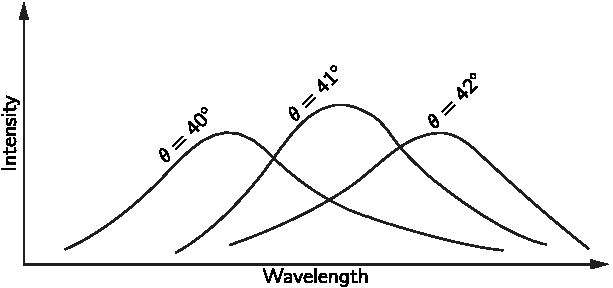
\includegraphics[width=0.9\linewidth]{fyz_fig0645.pdf}
      \caption{Intenzita elektromagnetických vln jako funkce vlnové délky pro tři úhly (měřené z 
               opačného směru, než je Slunce) pozorovaná pouze za určitých meteorologických 
               podmínek (\cite[s.~362]{Feynman02})}
      \label{fyz:fig0645}
    \end{figure}

    Avšak připadá nám graf na obr. \ref{fyz:fig0645} krásný? Obsahuje mnohem více podrobností, než
    vnímáme, když se díváme na duhu, neboť naše oči nedokážou vidět přesné podrobnosti ve tvaru
    spektra. Oko však vnímá duhu jako krásnou. Máme dostatek představivosti k tomu, abychom ve
    spektrálních křivkách viděli stejnou krásu jako vidíme, když se díváme přímo na duhu? Nevím.
    
    Ale představme si, že máme graf koeficientu odrazu krystalu chloridu sodného jako funkce vlnové
    délky v infračervené oblasti, a též i jako funkci úhlu. Dokázal bych si představit, jak by se to
    jevilo mým očím, kdyby mohly vidět v infračervené oblasti - snad nějaká jasná lesklá „zelená“,
    pomíchaná s odrazy od povrchu zbarvenými „kovově červeně“. To by byla překrásná věc, ale nevím,
    zda bych se mohl vůbec kdy podívat na graf koeficientu odrazu \ce{NaCl} naměřeného pomocí
    nějakého přístroje a prohlásit, že obsahuje stejnou krásu.
    
    Na druhé straně, i když nedokážeme vidět krásu v konkrétních naměřených výsledcích, můžeme vždy
    tvrdit, že vidíme určitou krásu v rovnicích popisujících obecné fyzikální zákony. Například, v
    případě rovnice \eqref{fyz:eq970} je cosi pěkného na té pravidelnosti, s jakou se v ní vyskytují
    \(x\), \(y\), \(z\) a \(t\). A tato překrásná symetrie ve výskytu \(x\), \(y\), \(z\) a \(t\)
    dává tušit ještě větší krásu, která se týká čtyř rozměrů, možnosti, že prostor se vyznačuje
    čtyřrozměrnou souměrností, možností tuto symetrii analyzovat a vypracovat přitom speciální
    teorii relativity (\ref{part:FYZV}). S rovnicemi je tedy spojeno dost intelektuální krásy.    

  \section{Kulové vlny}\label{fyz:IIchapXXsecIV}   
    Viděli jsme, že existují řešení vlnové rovnice, která příslušejí rovinným vlnám a že každou
    elektromagnetickou vlnu lze popsat jako superpozici mnoha rovinných vln. V určitých speciálních
    případech je však pohodlnější popisovat vlnové pole v jiném matematickém tvaru. Nyní bychom rádi
    probrali teorii kulových vln - vln odpovídajích kulovým plochám, které se rozbíhají z néjakého
    středu. Hodíme-li kámen do jezera, rozruch se šíří ve formé kruhových vln po hladině - jde o
    dvojrozměrné vlny. Kulová vlna je podobný útvar, jenže se šíří ve třech rozměrech.

    Dříve, než začneme s popisem kulových vln, potřebujeme trochu matematiky. Mějme funkci, která
    závisí pouze na radiální vzdálenosti \(r\) od určitého počátku - jinými slovy, funkci, která je
    kulově symetrická. Označme ji \(\psi(r)\), kde \(r\) znamená
    \begin{equation*}
      r=\sqrt{x^2+y^2+z^2},
    \end{equation*}
    tj. radiální vzdálenost od počátku soustavy souřadnic. Abychom zjistili, které funkce
    \(\psi(r)\) splňují vlnovou rovnici, budeme potřebovat výraz pro Laplaceův operátor funkce
    \(\psi\). Potřebujeme tedy najít součet druhých derivací \(\psi\) podle \(x\), \(y\) a \(z\).
    Budeme používat označení \(\psi'(r)\) pro derivaci \(\psi\) podle \(r\) a \(\psi''(r)\) pro
    druhou derivaci \(\psi\) podle \(r\).

    Nejdříve najdeme derivace podle \(x\). První derivace je
    \begin{equation*}
      \diffp{\psi(r)}{x}=\psi'(r)\,\diffp{r}{x}.
    \end{equation*}
    Druhá derivace \(\psi\) podle \(x\) je
    \begin{equation*}
      \diffp[2]{\psi}{x}=  \psi''\left(\diffp{r}{x}\right)^2 + \psi'\,\diffp[2]{r}{x}.
    \end{equation*}
    Parciální derivace \(r\) podle \(x\) lze vypočítat z těchto vztahů:
    \begin{equation*}
      \diffp{r}{x}=\frac{x}{r},\quad \diffp[2]{r}{x} = \dfrac{1}{r}\left(1-\dfrac{x^2}{r^2}\right).
    \end{equation*}
    Druhá derivace \(\psi\) podle \(x\) tedy bude
    \begin{subequations} 
      \begin{alignat}{3}
        \diffp[2]{\psi}{x} &=\dfrac{x^2}{r^2}\,        &&
          \psi''+ \dfrac{1}{r}\biggl(1-\dfrac{x^2}{r^2}&&\biggr)\psi'.  \label{fyz:eq989a} \\[1.5ex]
        \diffp[2]{\psi}{y} &= \dfrac{y^2}{r^2}\,       &&
          \psi''+ \dfrac{1}{r}\biggl(1-\dfrac{y^2}{r^2}&&\biggr)\psi',  \label{fyz:eq989b} \\[1.5ex]
        \diffp[2]{\psi}{z} &= \dfrac{z^2}{r^2}\,       &&
          \psi''+ \dfrac{1}{r}\biggl(1-\dfrac{z^2}{r^2}&&\biggr)\psi'.  \label{fyz:eq989c}
      \end{alignat}
    \end{subequations}
    Laplaceův operátor představuje součet těchto tří derivací. S ohledem na to, že
    \(x^2+y^2+z^2=r^2\), dostáváme tento vztah:
    \begin{equation}\label{fyz:eq995}
      \nabla^2\psi(r)=\psi''(r)+\dfrac{2}{r}\,\psi'(r).
    \end{equation}
    Často je vhodnější psát tento vztah v následujícím tvaru:
    \begin{equation}\label{fyz:eq991}
      \nabla^2\psi(r)=\dfrac{1}{r}\,\diff[2]{ }{r}(r\psi).
    \end{equation}
    Provedeme-li derivaci vyznačenou v \eqref{fyz:eq991}, přesvědčíme se, že výrazy na pravých
    stranách vztahů \eqref{fyz:eq995} a \eqref{fyz:eq991} jsou stejné.
    
    Chceme-li zkoumat kulově symetrická pole, která se mohou šířit ve formě kulových vln, musí
    veličina popisující pole být funkcí jak \(r\) tak i \(t\). Ptejme se tedy, jaké funkce \(\psi(r,
    t)\) jsou řešeními trojrozměrné vlnové rovnice
    \begin{equation}\label{fyz:eq992}
      \nabla^2\psi(r,t)-\dfrac{1}{c^2}\,\diffp[2]{ }{t}\,\psi(r,t)=0.
    \end{equation}
    Protože \(\psi(r, t)\) závisí na prostorových souřadnicích pouze prostřednictvím \(r\), můžeme
    pro Laplaceův operátor použít vztah \eqref{fyz:eq991}, který jsme už odvodili. Abychom však byli
    přesní, měli bychom derivace podle \(r\) psát jako parciální, neboť \(\psi\) je i funkcí \(t\).
    Vlnová rovnice pak získá tento tvar:
    \begin{equation*}
      \frac{1}{r}\,\diffp[2]{ }{r}\,(r\psi) - \dfrac{1}{c^2}\,\diffp[2]{ }{t}\,\psi=0.
    \end{equation*}
    Potřebujeme vyřešit tuto rovnici, která se zdá být mnohem složitější, než rovnice pro případ
    rovinných vln. Všimněme si však, že když ji vynásobíme \(r\), dostaneme
    \begin{equation}\label{fyz:eq993}
      \diffp[2]{ }{r}\,(r\psi) - \dfrac{1}{c^2}\,\diffp[2]{ }{t}\,(r\psi)=0.
    \end{equation}
    Podle této rovnice splňuje funkce \(r\psi\) jednorozměrnou vlnovou rovnici s proměnnou \(r\). Na
    základě obecného principu, který jsme tak často zdůrazňovali, že stejné rovnice mají stejná
    řešení, víme, že když je \(r\psi\)  funkcí pouze proměnné \((r - ct)\), bude řešením rovnice
    \eqref{fyz:eq993}. Víme tedy, že kulové vlny musí mít tvar
    \begin{equation*}
      r\psi(r,t)=f(r-ct).
    \end{equation*}
    Nebo, jak jsme viděli dřív, lze stejně dobře říci, že \(r\psi\) má tvar
    \begin{equation*}
      r\psi=f(t-\sfrac{r}{c}).
    \end{equation*}
    Po vydělení proměnnou \(r\) dostáváme výsledek, že veličina \(\psi\) popisující pole (ať už
    jakákoliv) má následující matematické vyjádření:
    \begin{equation}\label{fyz:eq994}
      \psi=\dfrac{f(t-\sfrac{r}{c})}{r}.
    \end{equation}
    Tato funkce představuje obecnou kulovou vlnu šířící se rychlostí \(c\) z počátku souřadnicové
    soustavy všemi směry. Odhlédneme-li na okamžik od \(r\) ve jmenovateli, má amplituda vlny jako
    funkce vzdálenosti od počátku určitý tvar, který postupuje rychlostí \(c\) ven, \(r\) ve
    jmenovateli však znamená, že amplituda vlny klesá s postupem vlny přímo úmémě \(\sfrac{1}{r}\).
    Jinými slovy, na rozdíl od rovinné vlny, v níž zůstává amplituda při pohybu vlny konstantní, v
    kulové vlně se amplituda neustále zmenšuje (obr. \ref{fyz:fig0649}). Tento jev lze snadno
    pochopit na základě jednoduchého fyzikálního důvodu.

    \begin{figure}[ht!] % \ref{fyz:fig0649}
      \centering
      \subcaptionbox{\(\psi\) jako funkce \(r\) při \(t = t_1\), a tatáž vlna v pozdějším čase
        \(t_2\) \label{fyz:fig0649a}}{\luafigure[0.9]{fyz_fig0649a.pdf}}                            \\
      \subcaptionbox{\(\psi\) jako funkce \(t\) pro \(r = r_1\) a tatáž vlna pozorovaná v poloze
        \(r_2\) \label{fyz:fig0649b}}{\luafigure[0.9]{fyz_fig0649b.pdf}}
      \caption{Kulová vlna \(\psi=f(t-\sfrac{r}{c})/r\). (\cite[s.~366]{Feynman02})}
      \label{fyz:fig0649}
    \end{figure}

    Víme, že hustota energie ve vlně závisí na druhé mocnině amplitudy vlny. Při postupu vlny se
    její energie rozptyluje na větší a větší plochu, která je přímo úměrná druhé mocnině vzdálenosti
    od středu. Když se celková energie zachovává, musí se hustota energie zároveň zmenšovat jako
    \(1/r^2\) a amplituda vlny tedy musí klesat jako \(1/r\). Takže vztah \eqref{fyz:eq994}
    představuje „rozumný“ výraz pro kulovou vlnu.
    
    Dosud jsme nevzali v úvahu druhé možné řešení vlnové rovnice:
    \begin{align*}
      r\psi &=g(t+r/c), \\
      \shortintertext{resp.}
      \psi  &=\dfrac{g\left(t + \sfrac{r}{c}\right)}{r}.
    \end{align*}
    Toto také představuje kulovou vlnu, ale takovou, která se pohybuje dovnitř, tj. od velkých
    vzdáleností \(r\) směrem k počátku souřadnicové soustavy.
    
    Nyní zavedeme jeden speciální předpoklad. Tvrdíme bez jakéhokoliv důkazu, že vlnami generovanými
    zdrojem jsou pouze ty vlny, které se pohybují směrem \emph{ven} ze zdroje. Protože víme, že vlny
    jsou způsobeny pohybem nábojů, musíme se domnívat, že vlny postupují od náboje pryč. Bylo by
    totiž dost divné představovat si, že dříve, než se náboje uvedly do pohybu, vystartovala z
    nekonečna kulová vlna a k nábojům dorazila právě v čase, když se začaly pohybovat. Je to možné
    řešení, ale zkušenost ukazuje, že jsou-li náboje urychlovány, pohybují se vlny od nábojů pryč.
    Ačkoli Maxwellovy rovnice připouštějí obě možnosti, přibereme k nim jako \emph{dodatečný fakt},
    založený na zkušenosti, že fyzikální smysl mají pouze řešení představující rozbíhavé vlny.
    
    Je však nutné poznamenat, že tento dodatečný předpoklad má zajímavý důsledek: jím jsme
    odstranili symetrii vzhledem k času, která existuje v Maxwellových rovnicích. Původní rovnice
    pro \(\vec{E}\) a \(\vec{B}\) a také vlnové rovnice, které jsme z nich odvodili, se vyznačují
    tím, že změníme-li znaménko \(t\), rovnice se nezmění. Podle těchto rovnic pro každé řešení
    odpovídající vlně pohybující se v jednom směru existuje stejně platné řešení znamenající vlnu
    pohybující se ve směru opačném. Naše tvrzení, že budeme brát v úvahu pouze vycházející vlny, je
    důležitým dodatečným předpokladem. (Pečlivě byla prozkoumána i taková formulace elektrodynamiky,
    v níž se tento předpoklad nezavádí. Je udivující, že v mnoha situacích nevede k fyzikálně
    absurdním důsledkům, ale hovořit nyní o těchto ideách by nás odvedlo příliš daleko od naší
    cesty. Trochu víc o nich povíme v kapitole \ref{fyz:IIchapXXIIX}.)

    Musíme se zmínit ještě o jedné důležité věci. V našem řešení \eqref{fyz:eq994} pro rozbíhavou
    vlnu je v počátku souřadnicové soustavy funkce \(\psi\) nekonečná. To je trochu neobvyklé.
    Raději bychom měli takové vlnové řešení, které by bylo hladké všude. Naše řešení musí fyzikálně
    představovat situaci, v níž se v počátku soustavy souřadnic nachází nějaký zdroj. Jinak řečeno,
    nedopatřením jsme se dopustili chyby. Rovnici volných vln \eqref{fyz:eq992} s nulou na pravé
    straně jsme nevyřešili všudey ale s výjimkou počátku souřadnicové soustavy. Chyba se nám vetřela
    proto, že některé kroky v našem odvození nejsou při \(r = 0\) „dovoleny“.
    
    Ukážeme, jak snadno se v elektrostatické úloze taková chyba udělá. Představme si, že potřebujeme
    najít řešení rovnice pro elektrostatický potenciál \(\nabla^2\varphi = 0\). Laplaceův operátor
    funkce \(\varphi\) je roven nule, neboť jsme předpokládali, že nikde nejsou žádné náboje. Ale
    jak je to s kulově symetrickým řešením této rovnice, tj. když je nějaká funkce \(\varphi\)
    závislá jen na \(r\)? Použijeme-li pro Laplaceův operátor vztah \eqref{fyz:eq991}, dostaneme
    \begin{equation*}
      \dfrac{1}{r}\,\diff[2]{ }{r}\,(r\varphi)=0.
    \end{equation*}
    Vynásobením této rovnice proměnnou \(r\) dostáváme rovnici, kterou lze bezprostředně integrovat:
    \begin{equation*}
      \diff[2]{ }{r}\,(r\varphi)=0.
    \end{equation*}
    Integrujeme-li jednou podle \(r\) zjistíme, že první derivace funkce \(r\varphi\) je rovna
    konstantě, kterou můžeme označit \(a\):
    \begin{equation*}
      \diff{}{r}\,(r\varphi)=a.
    \end{equation*}
    Opětovným integrováním dostaneme, že funkce \(r\varphi\) má tento tvar:
    \begin{equation*}
      r\varphi=ar+b,
    \end{equation*}
    kde \(b\) je další integrační konstanta. Následující \(\varphi\) jsme tedy našli jako řešení
    rovnice pro elektrostatický potenciál ve vakuu:
    \begin{equation*}
      \varphi=a+\dfrac{b}{r}.
    \end{equation*}

    Něco je zde zřejmě chybné. Víme, jak vypadá řešení pro elektrostatický potenciál v oblasti, kde
    žádné elektrické náboje nejsou: potenciál je všude roven konstantě. Odpovídá to prvnímu sčítanci
    v našem řešení. Ale my máme i druhý člen, podle něhož existuje ještě příspěvek k potenciálu
    měnící se jako převrácená hodnota vzdálenosti od počátku souřadnicové soustavy. Víme však, že
    takový potenciál přísluší bodovému náboji nacházejícímu se v počátku soustavy. Ačkoliv se nám
    tedy zdálo, že hledáme řešení pro potenciál ve vakuu, nalezené řešení nám poskytuje i pole pro
    bodový náboj v počátku vztažné soustavy. Zjišťujeme podobnost mezi tím, co se stalo nyní a co se
    stalo tehdy, když jsme hledali kulově symetrické řešení vlnové rovnice? Kdyby v počátku soustavy
    reálně neexistovaly žádné náboje nebo proudy, nebyly by ani kulové rozbíhavé vlny. Kulové vlny
    musí být vytvářeny zdroji nacházejícími se v počátku. V následující kapitole budeme zkoumat
    souvislost mezi rozbíhavými elektromagnetickými vlnami na jedné straně a proudy a napětími,
    které je vytváří, na straně druhé.


  \section{Příklady a cvičení}\label{fyz:IIchapXXsecV}

%---------------------------------------------------------------------------------------------------